\chapter{Siêu điện tích, tính đóng và siêu không gian}

\lectureoverview{Siêu đối xứng khó không phải vì các quy tắc của nó nhiều, mà vì các quy tắc ấy nối kết những ý niệm mà vật lý thông thường giữ tách rời. Ta bắt đầu với các biến Grassmann, mà các phần tử lẻ của chúng phản giao hoán và các hàm của chúng dừng lại sau hữu hạn hạng. Đại số đạo hàm của chúng sau đó cung cấp mô hình cho các bộ sinh đối xứng lẻ. Một dao động tử boson và một dao động tử fermion cho các siêu điện tích đơn giản nhất: phản giao hoán tử của chúng là Hamiltonian, vì vậy việc trao đổi boson và fermion gắn liền không thể tách rời với phép tịnh tiến theo thời gian. Cùng đại số đó cũng có thể được biểu diễn hình học bằng các phép tịnh tiến theo các phương Grassmann của một không-thời gian mở rộng gọi là siêu không gian.}

\section{Vì sao ta phải lùi lại trước khi tiến lên}

Siêu đối xứng là một trong những cấu trúc trừu tượng nhất của vật lý. Nó giống các phép quay và các phép tịnh tiến vì nó là một đối xứng, nhưng nó không nằm gọn trong không-thời gian thông thường nếu không mở rộng điều ta gọi là một tọa độ. Các tham số tự nhiên của nó là các đại lượng Grassmann: những đối tượng có thể cộng và nhân, nhưng phản giao hoán thay vì giao hoán.

Đó là lý do vì sao việc lao thẳng vào đại số cuối cùng sẽ không hữu ích. Trước hết ta sẽ làm cho phép tính lẻ trở nên dùng được, rồi nhắc lại cách các đối xứng liên tục thông thường được tổ chức, và chỉ sau đó mới kết hợp hai ý tưởng ấy. Lộ trình này dài hơn, nhưng mỗi bước đều chuẩn bị cho bước tiếp theo.

\section{Dạng thao tác của đại số Grassmann}

\subsection{Phần tử lẻ và phần tử chẵn}

Hãy để \(\epsilon_i\) ký hiệu các bộ sinh Grassmann độc lập. Chúng thỏa mãn
\begin{equation}
\epsilon_i\epsilon_j=-\epsilon_j\epsilon_i,
\qquad
\{\epsilon_i,\epsilon_j\}=0.
\end{equation}
Đặt \(i=j\), ta được
\begin{equation}
2\epsilon_i^2=0,
\qquad
\epsilon_i^2=0,
\end{equation}
trên trường số thực hoặc số phức. Bộ sinh không bằng không; chỉ có bình phương của nó bằng không.

Mỗi phần tử thuần nhất có một độ chẵn lẻ. Một tích chứa số lẻ các bộ sinh Grassmann là lẻ, còn một tích chứa số chẵn bộ sinh là chẵn:
\begin{align}
\text{odd}\times\text{odd}&=\text{even},\\
\text{odd}\times\text{even}&=\text{odd},\\
\text{even}\times\text{even}&=\text{even}.
\end{align}
Các phần tử chẵn giao hoán với các phần tử thuần nhất. Hai phần tử lẻ phản giao hoán. Do đó
\begin{equation}
n\epsilon_i=\epsilon_i n,
\qquad
\epsilon_i\epsilon_j=-\epsilon_j\epsilon_i,
\end{equation}
khi \(n\) là chẵn.

Một phần tử chẵn không nhất thiết là một số thực hay số phức thông thường. Chẳng hạn, tích \(\epsilon_1\epsilon_2\) là chẵn và lũy linh. Các số thông thường tạo thành phần vô hướng của đại số, còn các tích chẵn cung cấp thêm những phần tử giao hoán.

\begin{classroomqa}
\audiencequestion{Có sự phân biệt nào giữa đại số Grassmann và các số Grassmann không, hay chúng là cùng một thứ? \lecturetimestamp{00:06:45}}
\lecturerresponse{Các phần tử là các số Grassmann; còn đại số là tập hợp các phần tử ấy cùng với các quy tắc cộng và nhân của chúng. Vì thế ta có thể nói một cách lỏng là cùng một đối tượng, nhưng vẫn hữu ích khi phân biệt những thứ đang được thao tác với các quy tắc chi phối các thao tác ấy.}
\end{classroomqa}

\subsection{Các hàm dừng lại}

Một hàm của một biến Grassmann chỉ có hai lũy thừa khả dĩ:
\begin{equation}
f(\epsilon)=a+b\epsilon.
\end{equation}
Không có hạng \(\epsilon^2\). Với hai bộ sinh độc lập,
\begin{equation}
f(\epsilon_1,\epsilon_2)
=a+b_1\epsilon_1+b_2\epsilon_2+c\epsilon_1\epsilon_2.
\end{equation}
Khai triển dừng lại sau khi cả hai bộ sinh đã xuất hiện. Với \(n\) bộ sinh độc lập, các đơn thức có thứ tự tạo thành một cơ sở \(2^n\) chiều:
\begin{equation}
1,\quad
\epsilon_i,\quad
\epsilon_i\epsilon_j,\quad
\ldots,\quad
\epsilon_1\epsilon_2\cdots\epsilon_n.
\end{equation}
\editorialnote{Phát biểu hữu hạn chiều \(2^n\) là khuôn mẫu tổng quát đứng sau các ví dụ một và hai bộ sinh. Cũng có thể định nghĩa một đại số Grassmann vô hạn, nhưng mọi đa thức dùng ở đây đều chỉ liên quan đến hữu hạn bộ sinh.}

Khi hai bộ sinh thực được ghép thành một cặp phức \(\theta,\bar\theta\), với một quy ước thứ tự đã chọn, một hàm tổng quát có thể viết thành
\begin{equation}
f(\theta,\bar\theta)
=a+\bar b\,\theta+\bar\theta\,b+c\,\bar\theta\theta.
\end{equation}
Dấu gạch trên biểu thị ký hiệu cặp phức dùng ở đây. Đảo thứ tự ở hạng cuối làm đổi dấu:
\begin{equation}
\bar\theta\theta=-\theta\bar\theta.
\end{equation}

Thường sẽ thuận tiện nếu gán cho toàn bộ hàm một độ chẵn lẻ xác định. Nếu \(f\) là chẵn, thì \(a\) và \(c\) là chẵn, còn \(b\) và \(\bar b\) là lẻ. Nếu \(f\) là lẻ, các gán đó đảo lại. Bản thân các hệ số cũng có thể thuộc về một đại số Grassmann lớn hơn, miễn là chúng không phụ thuộc vào chính những biến mà theo đó ta đang khai triển.

\begin{classroomqa}
\audiencequestion{Có thể đưa một biến Grassmann vào các hàm lượng giác hay các hàm giải tích khác không? \lecturetimestamp{00:11:06}}
\lecturerresponse{Có, nhưng chuỗi lũy thừa dừng lại ngay lập tức. Với một bộ sinh lẻ,
\[
\sin\epsilon=\epsilon,\qquad
\cos\epsilon=1,\qquad
e^\epsilon=1+\epsilon.
\]
Tên gọi quen thuộc vẫn giữ nguyên, nhưng có quá ít lũy thừa để các hàm ấy phát triển độ phức tạp giải tích thường thấy của chúng.}
\end{classroomqa}

\section{Phép đạo hàm là việc theo dõi dấu}

Ta dùng đạo hàm Grassmann trái. Các quy tắc cục bộ xác định của nó là
\begin{equation}
\partial_\theta a=0,
\qquad
\partial_\theta(\theta B)=B,
\end{equation}
khi \(a\) và \(B\) độc lập với \(\theta\). Trước khi lấy đạo hàm, hãy chuyển \(\theta\) tương ứng sang bên trái. Mỗi lần đi qua một thừa số lẻ khác thì dấu đổi.

Chẳng hạn, nếu \(b\) là lẻ,
\begin{equation}
b\theta=-\theta b,
\qquad
\partial_\theta(b\theta)=-b.
\end{equation}
Không có điều gì bí ẩn xảy ra với đạo hàm. Dấu trừ xuất hiện trước khi lấy đạo hàm, khi các thừa số lẻ được sắp lại thứ tự.

\subsection{Phép tính hai biến}

Quay lại
\begin{equation}
f(\theta,\bar\theta)
=a+\bar b\,\theta+\bar\theta\,b+c\,\bar\theta\theta.
\end{equation}
Trước hết giả sử \(f\) là chẵn. Khi đó \(\bar b\) là lẻ và \(c\) là chẵn. Sắp lại thứ tự các hạng có chứa \(\theta\),
\begin{align}
\bar b\,\theta&=-\theta\bar b,\\
c\,\bar\theta\theta&=-\theta c\,\bar\theta.
\end{align}
Do đó
\begin{equation}
\partial_\theta f=-\bar b-c\bar\theta.
\end{equation}

Nếu \(f\) là lẻ, thì \(\bar b\) là chẵn và \(c\) là lẻ. Hạng đầu không đi qua hệ số lẻ nào, còn \(\theta\) ở hạng cuối đi qua hai thừa số lẻ, \(c\) và \(\bar\theta\). Hai dấu triệt tiêu nhau:
\begin{equation}
\partial_\theta f=\bar b+c\bar\theta.
\end{equation}

\begin{classroomqa}
\audiencequestion{Vì sao trong ví dụ chẵn, cả hai hạng còn lại đều mang dấu trừ? \lecturetimestamp{00:16:49}}
\lecturerresponse{Dấu thứ nhất xuất phát từ việc chuyển \(\theta\) qua hệ số lẻ \(\bar b\). Ở hạng cuối, \(c\) là chẵn, nhưng \(\theta\) phải đi qua biến lẻ \(\bar\theta\). Mỗi lần sắp lại như vậy đều đi qua một thừa số lẻ, nên mỗi lần đều sinh ra một dấu trừ.}
\end{classroomqa}

Câu trả lời phụ thuộc vào quy ước thứ tự, nhưng toán học thì không. Nếu ta bắt đầu từ \(c\theta\bar\theta\) thay vì \(c\bar\theta\theta\), hệ số được viết ra sẽ khác nhau bởi một dấu và công thức đạo hàm cũng sẽ thay đổi tương ứng.

\begin{classroomqa}
\audiencequestion{Hạng cuối có thể được viết với \(\theta\) và \(\bar\theta\) theo thứ tự đảo lại không, và dấu xuất hiện khi đó có ý nghĩa sâu hơn nào không? \lecturetimestamp{00:18:50}}
\lecturerresponse{Có thể viết theo một trong hai thứ tự, nhưng hoán đổi hai biến lẻ làm đổi dấu. Ta có thể hấp thụ dấu ấy vào hệ số \(c\). Ở giai đoạn này, hiệu ứng đó chỉ là chuyện ghi sổ: thứ tự có ý nghĩa, độ chẵn lẻ không đổi, và việc đổi dấu không bao giờ biến một đối tượng lẻ thành một đối tượng chẵn. Ý nghĩa vật lý xuất hiện khi chính việc ghi sổ ấy áp đặt thống kê fermion và siêu đối xứng.}
\end{classroomqa}

\begin{classroomqa}
\audiencequestion{Các hệ số \(a,b,c\) có đơn giản chỉ lấy từ trường số phức không? \lecturetimestamp{00:20:47}}
\lecturerresponse{Chúng có thể là các số phức thông thường khi độ chẵn lẻ mà chúng cần có là chẵn, nhưng chúng cũng có thể chứa các bộ sinh khác ngoài \(\theta,\bar\theta\). Đại số được quan tâm ở đây thông thường chứa mọi vô hướng phức cùng với một tập các bộ sinh lẻ được chọn và các tích của chúng.}
\end{classroomqa}

\begin{classroomqa}
\audiencequestion{Đạo hàm của các hàm chẵn và lẻ trông như đối nhau. Có phải đó là một đối xứng tổng quát không? \lecturetimestamp{00:22:31}}
\lecturerresponse{Không, tự nó không phải vậy. Các dấu xuất hiện một cách cơ học từ độ chẵn lẻ của từng hệ số và số thừa số lẻ bị đi qua. Đôi khi hai đáp án tình cờ đối nhau, nhưng quy tắc đáng tin cậy thì đơn giản hơn: mỗi lần trao đổi hai đối tượng lẻ đều đóng góp một dấu trừ.}
\end{classroomqa}

\subsection{Tọa độ và đạo hàm như các toán tử}

Có một phép tương tự thông thường rất gợi mở. Hãy để phép nhân với \(x\) và phép đạo hàm theo \(x\) tác dụng lên một hàm tùy ý \(g(x)\). Khi đó
\begin{align}
\partial_x\!\left(xg\right)&=g+xg',\\
x\partial_xg&=xg',
\end{align}
nên
\begin{equation}
[\partial_x,x]g=g.
\end{equation}
Vì điều này đúng với mọi \(g\),
\begin{equation}
[\partial_x,x]=1.
\end{equation}
Với \(p=-i\partial_x\), đây là đại số vị trí-xung lượng quen thuộc, trong hệ đơn vị \(\hbar=1\).

Phép tương tự Grassmann dùng một phản giao hoán tử. Lấy
\begin{equation}
f(\theta)=a+\theta b,
\end{equation}
với \(a\) chẵn và \(b\) lẻ, để \(f\) là chẵn. Trước hết,
\begin{equation}
\theta\partial_\theta f=\theta b.
\end{equation}
Theo thứ tự ngược lại,
\begin{align}
\partial_\theta(\theta f)
&=\partial_\theta(\theta a+\theta^2b)\\
&=a.
\end{align}
Cộng hai thứ tự lại cho chính hàm ban đầu:
\begin{equation}
\left(\partial_\theta\theta+\theta\partial_\theta\right)f
=a+\theta b=f.
\end{equation}
Do đó
\begin{equation}
\boxed{\{\partial_\theta,\theta\}=1.}
\end{equation}
Bản thân đạo hàm \(\partial_\theta\) là lẻ. Đó là lý do vì sao quan hệ chính tắc của nó với tọa độ lẻ là một phản giao hoán tử.

\begin{classroomqa}
\audiencequestion{Có thể dùng một hàm chứa cả phần chẵn lẫn phần lẻ thay vì gán một độ chẵn lẻ xác định không? \lecturetimestamp{00:31:05}}
\lecturerresponse{Có thể tạo ra những phần tử không thuần nhất như vậy, nhưng các phép tính thông thường được tổ chức theo các đối tượng thuần nhất chẵn và lẻ. Một độ chẵn lẻ xác định làm cho mọi dấu trong một tích có phân bậc đều không mơ hồ; một đối tượng trộn được xử lý bằng cách tách nó thành phần chẵn và phần lẻ.}
\end{classroomqa}

\begin{classroomqa}
\audiencequestion{Trong phép tính giao hoán tử thông thường, hàm thử \(g(x)\) có được giả sử là lẻ không? \lecturetimestamp{00:31:45}}
\lecturerresponse{Không. Đó là một hàm thông thường của một tọa độ giao hoán thông thường. Nó chỉ được đưa vào để chỉ ra cách chứng minh đồng nhất thức toán tử \([\partial_x,x]=1\) trước khi lặp lại lập luận với cặp Grassmann \(\partial_\theta,\theta\).}
\end{classroomqa}

\begin{classroomqa}
\audiencequestion{Có giới hạn nào cho số bộ sinh Grassmann độc lập không? \lecturetimestamp{00:32:16}}
\lecturerresponse{Không có giới hạn trên về mặt đại số. Với \(n\) bộ sinh, cơ sở có \(2^n\) đơn thức, nên phần ghi sổ tăng rất nhanh, nhưng bản thân phép xây dựng vẫn hoạt động với mọi \(n\) hữu hạn.}
\end{classroomqa}

\subsection{Phép tích phân}

Tích phân trên một biến Grassmann được xác định bởi
\begin{equation}
\int d\theta\,1=0,
\qquad
\int d\theta\,\theta=1.
\end{equation}
Do đó, với \(f(\theta)=a+\theta b\),
\begin{equation}
\int d\theta\,f(\theta)=b=\partial_\theta f(\theta).
\end{equation}
Vì vậy phép tích phân và phép đạo hàm thực hiện cùng một phép trích xuất thành phần. Đây là tích phân Berezin. Chuẩn hóa của nó là lựa chọn đơn giản duy nhất tương thích với bất biến tịnh tiến và phép tích phân từng phần Grassmann. \editorialnote{Các quy tắc thành phần diễn đạt chính xác nhận định của bài giảng rằng tích phân và đạo hàm Grassmann là cùng một phép toán.}

\section{Đối xứng thông thường làm mốc chuẩn}

Xét một nhóm unita liên tục với các bộ sinh Hermite \(G_i\). Gần phần tử đơn vị,
\begin{equation}
U(\alpha)=\mathbf 1+i\alpha^iG_i+O(\alpha^2),
\end{equation}
trong đó \(\alpha^i\) là các tham số giao hoán thông thường. Quy luật nhân vô cùng bé được mã hóa bởi đại số Lie
\begin{equation}
[G_i,G_j]=i f_{ij}{}^{k}G_k.
\end{equation}
Các hằng số \(f_{ij}{}^k\) là các hằng số cấu trúc. Tính đóng nghĩa là giao hoán hai bộ sinh bất kỳ sẽ cho lại một tổ hợp tuyến tính của các bộ sinh đã có trong đại số.

Đối với các phép quay,
\begin{equation}
[L_i,L_j]=i\varepsilon_{ijk}L_k.
\end{equation}
Ba thành phần Hermite có thể được kết hợp thành các toán tử bậc thang không Hermite
\begin{equation}
L_\pm=L_x\pm iL_y,
\end{equation}
chúng nâng hoặc hạ số lượng tử từ \(m\) đi một đơn vị. Các tổ hợp phức vẫn hữu ích mà không làm thay đổi tính Hermite của các bộ sinh vật lý nền tảng.

Trong một cơ sở tổng quát, chỉ hai chỉ số đầu của \(f_{ij}{}^k\) buộc phải phản đối xứng. Với một đại số compact có metric trực chuẩn bất biến, ta có thể hạ chỉ số cuối và chọn các quy ước sao cho \(f_{ijk}\) là phản đối xứng hoàn toàn, như trong trường hợp phép quay. \editorialnote{Lưu ý này tách biệt tính phản đối xứng phổ quát của giao hoán tử với tính chất mạnh hơn có được trong cơ sở quay quen thuộc.}

Để \(G_i\) sinh ra một đối xứng thực sự của một hệ không phụ thuộc thời gian,
\begin{equation}
[H,G_i]=0.
\end{equation}
Tương đương, \(G_i\) ánh xạ mọi không gian riêng của năng lượng vào chính nó. Khi không có phụ thuộc thời gian tường minh, phương trình Heisenberg cho
\begin{equation}
\frac{dG_i}{dt}=i[H,G_i]=0,
\end{equation}
vì thế bộ sinh là một điện tích bảo toàn.

Các đại lượng quan sát thông thường là chẵn. Một trường fermion là lẻ, nhưng một trường lẻ cô lập tự nó không phải là một đại lượng quan sát đo được; các toán tử vật lý chứa tổng số chẵn các thừa số fermion. Siêu đối xứng làm thay đổi độ chẵn lẻ của các bộ sinh, chứ không thay đổi độ chẵn lẻ mà các kết quả quan sát được phải có.

Ký hiệu gọn gàng cho mọi trường hợp là giao hoán tử phân bậc
\begin{equation}
[X,Y]_{\mathrm{gr}}
=XY-(-1)^{|X||Y|}YX.
\end{equation}
Nó là giao hoán tử thông thường nếu một trong hai toán tử là chẵn, và là phản giao hoán tử nếu cả hai đều lẻ.

\section{Dao động tử siêu đối xứng nhỏ nhất}

\subsection{Một mode boson và một mode fermion}

Xét một mode boson đơn với các toán tử tạo và hủy \(a_+\) và \(a_-\):
\begin{equation}
[a_-,a_+]=1,
\qquad
[a_+,a_+]=[a_-,a_-]=0.
\end{equation}
Toán tử số của nó là
\begin{equation}
N_B=a_+a_-,
\end{equation}
và số chiếm cứ của nó có thể là \(0,1,2,\ldots\).

Đối với một mode fermion đơn, đưa vào \(c_+\) và \(c_-\):
\begin{equation}
\{c_-,c_+\}=1,
\qquad
\{c_+,c_+\}=\{c_-,c_-\}=0.
\end{equation}
Do đó
\begin{equation}
c_+^2=c_-^2=0,
\qquad
N_F=c_+c_-,
\end{equation}
và số chiếm cứ chỉ có thể là \(0\) hoặc \(1\). Các toán tử boson là chẵn, các toán tử fermion là lẻ, và mọi \(a_\pm\) đều giao hoán với mọi \(c_\pm\).

\editorialnote{Tính lũy linh này giới hạn mode fermion vào một trạng thái chiếm cứ. Mode boson có số chiếm cứ không bị hạn chế; một câu nói thoáng qua theo chiều ngược lại trong phần thảo luận trên lớp được chính đại số dao động tử giải quyết.}

Giả sử boson và fermion có cùng năng lượng nghỉ \(m\), và định nghĩa
\begin{equation}
Q=\sqrt m\,a_+c_-,
\qquad
\bar Q=Q^\dagger=\sqrt m\,a_-c_+.
\end{equation}
Toán tử \(Q\) hủy một fermion và tạo một boson. Liên hợp của nó hủy một boson và tạo một fermion. Mỗi toán tử chứa một toán tử fermion và vì thế là lẻ.

Trên các trạng thái số, tác dụng của chúng được viết tường minh:
\begin{align}
Q\ket{n,1}
&=\sqrt{m(n+1)}\,\ket{n+1,0},
&
Q\ket{n,0}&=0,\\
\bar Q\ket{n,0}
&=\sqrt{mn}\,\ket{n-1,1},
&
\bar Q\ket{n,1}&=0.
\end{align}
\editorialnote{Các công thức trạng thái số là dạng chuẩn hóa trực tiếp của tác dụng thay thế hạt được mô tả trong bài giảng.}

\subsection{Phản giao hoán tử khép kín trên năng lượng}

Phiên bản phân bậc tương ứng với việc tìm một đại số Lie là tính
\begin{align}
\{Q,\bar Q\}
&=Q\bar Q+\bar Q Q\\
&=m\left(a_+c_-a_-c_+
        +a_-c_+a_+c_-\right).
\end{align}
Vì các \(a\) là chẵn, chúng đi qua các \(c\) mà không sinh dấu:
\begin{equation}
\{Q,\bar Q\}
=m\left(a_+a_-c_-c_+
        +a_-a_+c_+c_-\right).
\end{equation}
Bây giờ dùng
\begin{equation}
c_-c_+=1-c_+c_-,
\qquad
a_-a_+=a_+a_-+1.
\end{equation}
Khi đó
\begin{align}
\{Q,\bar Q\}
&=m\left[
N_B(1-N_F)+(N_B+1)N_F
\right]\\
&=m(N_B+N_F).
\end{align}
Hệ số 2 phụ thêm tạm thời xuất hiện trong lúc sắp xếp lại trực tiếp sẽ biến mất: một đóng góp cho \(N_B\), đóng góp kia cho \(N_F\).

Đối với các hạt đứng yên có cùng khối lượng, Hamiltonian là
\begin{equation}
H=m(N_B+N_F).
\end{equation}
Do đó
\begin{equation}
\boxed{\{Q,\bar Q\}=H.}
\end{equation}

\begin{figure}[H]
\centering
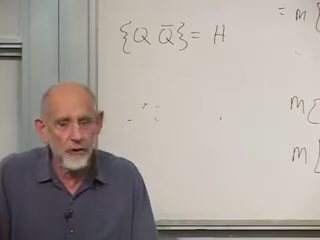
\includegraphics[width=0.62\textwidth]{lecture_05_figure_02.png}
\lectureframe{00:55:46.300}
\caption{Hệ thức khép kín trung tâm được tách riêng trên bảng. Có thể nhìn thấy các dấu ngoặc nhọn và \(Q,\bar Q,H\); dấu phẩy được bổ sung bởi ký hiệu phản giao hoán tử chuẩn.}
\end{figure}

Mốc 0 của năng lượng đã được chọn sao cho trạng thái rỗng có \(H=0\). Trong dao động tử siêu đối xứng, đây là quy ước tự nhiên: các đóng góp năng lượng không điểm của boson và fermion triệt tiêu nhau. \editorialnote{Bài giảng làm việc trực tiếp với tổng năng lượng nghỉ và không viết riêng các hạng không điểm; quy ước đã nêu làm cho lựa chọn đó trở nên tường minh.}

Hamiltonian là chẵn. Nó cũng là một bộ sinh đối xứng: nó sinh ra các phép tịnh tiến theo thời gian. Vì vậy, các bộ sinh lẻ không khép kín chỉ giữa chúng với nhau trừ phi bộ sinh chẵn của phép tịnh tiến thời gian được bao gồm.

\begin{classroomqa}
\audiencequestion{Vế nào của hệ thức là chẵn? Có phải Hamiltonian không? \lecturetimestamp{00:58:24}}
\lecturerresponse{Đúng. Năng lượng là một đại lượng quan sát thông thường, nên \(H\) là chẵn. Siêu điện tích \(Q\) là lẻ, và tích của hai đại lượng lẻ là chẵn; do đó \(\{Q,\bar Q\}\) có thể bằng \(H\). Một bộ sinh lẻ và một bộ sinh chẵn liên hệ với nhau bằng giao hoán tử, không phải phản giao hoán tử.}
\end{classroomqa}

\subsection{Hoàn tất đại số}

Các hệ thức cùng chẵn lẻ suy ra ngay:
\begin{equation}
\{Q,Q\}=2Q^2=0,
\qquad
\{\bar Q,\bar Q\}=2\bar Q^2=0,
\end{equation}
vì \(Q^2\) chứa \(c_-^2\) và \(\bar Q^2\) chứa \(c_+^2\).

Điều còn lại là hệ thức với \(H\). Đặt
\begin{equation}
H\ket{E}=E\ket{E}.
\end{equation}
Nếu khối lượng của boson và fermion bằng nhau, \(Q\) thay hạt này bằng hạt kia mà không đổi năng lượng. Do đó \(Q\ket{E}\) bằng không hoặc là một trạng thái riêng khác với cùng trị riêng:
\begin{equation}
H Q\ket{E}=E Q\ket{E}.
\end{equation}
Mặt khác,
\begin{equation}
QH\ket{E}=Q(E\ket{E})=E Q\ket{E}.
\end{equation}
Lấy hiệu,
\begin{equation}
[H,Q]\ket{E}=0.
\end{equation}
Nếu các trạng thái riêng năng lượng tạo thành một cơ sở đầy đủ, thì điều này đúng như một đồng nhất thức toán tử:
\begin{equation}
[H,Q]=0,
\qquad
[H,\bar Q]=0.
\end{equation}

\begin{classroomqa}
\audiencequestion{Điều gì xảy ra nếu boson và fermion không có cùng khối lượng? \lecturetimestamp{01:01:16}}
\lecturerresponse{Khi đó việc thay hạt này bằng hạt kia làm đổi năng lượng, nên siêu điện tích được đề xuất không giao hoán với Hamiltonian và siêu đối xứng đơn giản bị mất. Với
\[
H=m_BN_B+m_FN_F,
\]
kết quả tường minh là
\[
[H,Q]=(m_B-m_F)Q.
\]
Nó triệt tiêu đúng khi \(m_B=m_F\). \editorialnote{Giao hoán tử trong trường hợp khối lượng không bằng nhau là dạng toán tử trực tiếp của lập luận thay đổi năng lượng và làm cho điều kiện khối lượng bằng nhau trở nên tường minh.}}
\end{classroomqa}

\begin{classroomqa}
\audiencequestion{Có thể lặp lại chậm hơn lập luận dùng trạng thái riêng năng lượng không? \lecturetimestamp{01:01:37}}
\lecturerresponse{Bắt đầu với \(H\ket{E}=E\ket{E}\). Khối lượng bằng nhau ngụ ý rằng \(Q\ket{E}\) có cùng năng lượng xác định \(E\), nên \(HQ\ket{E}=EQ\ket{E}\). Theo thứ tự kia ta được \(QH\ket{E}=QE\ket{E}=EQ\ket{E}\), vì \(E\) là một vô hướng thông thường. Hiệu của chúng triệt tiêu trên mọi trạng thái riêng năng lượng. Tính đầy đủ khi đó nâng phát biểu từ các trạng thái ấy lên phương trình toán tử \([H,Q]=0\).}
\end{classroomqa}

Vì thế, đại số mô hình đồ chơi đầy đủ là
\begin{align}
\{Q,\bar Q\}&=H,\\
\{Q,Q\}&=\{\bar Q,\bar Q\}=0,\\
[H,Q]&=[H,\bar Q]=0.
\end{align}
Các siêu điện tích là những điện tích lẻ bảo toàn. Điều đáng ngạc nhiên hơn là đại số của chúng trộn một phép toán làm đổi loại hạt với bộ sinh của phép tịnh tiến trong không-thời gian.

\section{Vì sao Hamiltonian tương ứng với phép tịnh tiến theo thời gian}

Trong mô hình rút gọn này không có tọa độ không gian, nhưng có thời gian. Phương trình Schrödinger là
\begin{equation}
i\frac{\partial}{\partial t}\ket{\psi(t)}
=H\ket{\psi(t)}.
\end{equation}

\begin{figure}[H]
\centering
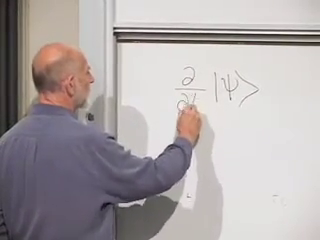
\includegraphics[width=0.56\textwidth]{lecture_05_figure_03.png}
\lectureframe{01:07:26.300}
\caption{Đạo hàm theo thời gian được viết bên cạnh \(\ket{\psi}\). Bàn tay che khuất một phần mẫu số; phương trình Schrödinger đầy đủ đã được cho ở trên.}
\end{figure}

Đối với một độ dời hữu hạn \(\delta\),
\begin{equation}
\ket{\psi(t+\delta)}
=e^{-iH\delta}\ket{\psi(t)}.
\end{equation}
Khai triển đến bậc nhất,
\begin{equation}
\ket{\psi(t+\delta)}
=\left(\mathbf 1-i\delta H\right)\ket{\psi(t)}
+O(\delta^2).
\end{equation}
Vì vậy \(H\) là bộ sinh vô cùng bé làm tiến hóa một trạng thái theo thời gian.

Các đối xứng nội tại như isospin và màu cũng làm đổi nhãn hạt. Isospin có thể trộn các trạng thái proton và neutron; các phép quay màu trộn các quark đỏ, lục và lam. Tuy vậy, không một hợp thành nào của các biến đổi nội tại ấy tịnh tiến một hệ trong không gian hay thời gian. Siêu đối xứng thì khác:
\begin{equation}
\begin{gathered}
\text{odd particle-changing transformation}\\
\mathrel{\stackrel{\{\ ,\ \}}{\Longrightarrow}}\\
\text{time translation}
\end{gathered}
\end{equation}
Đó là đầu mối cho thấy bản thân các bộ sinh lẻ có thể là các phép tịnh tiến, nhưng dọc theo những tọa độ khác với các tọa độ thông thường.

\section{Siêu không gian}

\subsection{Một hàm của thời gian và các tọa độ lẻ}

Đưa vào một hàm
\begin{equation}
\Psi=\Psi(\theta,\bar\theta,t).
\end{equation}
Nó có thể được xem như một hàm sóng trong mô hình đồ chơi hoặc, tổng quát hơn, như một siêu trường. Vì khai triển theo các biến lẻ kết thúc hữu hạn,
\begin{equation}
\Psi(\theta,\bar\theta,t)
=A(t)+\bar\chi(t)\theta
+\bar\theta\chi(t)+F(t)\bar\theta\theta.
\end{equation}
Đối tượng duy nhất này chứa gộp các hàm thành phần chẵn và lẻ. \editorialnote{Khai triển theo thành phần này áp dụng đa thức Grassmann đã được xây dựng trước đó; đó là nội dung tường minh chuẩn của một hàm trên siêu không gian đồ chơi này.}

Một phép tịnh tiến thời gian thông thường giữ \(\theta,\bar\theta\) cố định và biến
\begin{equation}
t\longmapsto t+\delta.
\end{equation}
Đến bậc nhất,
\begin{equation}
\Psi(\theta,\bar\theta,t+\delta)
=\Psi(\theta,\bar\theta,t)
+\delta\,\partial_t\Psi(\theta,\bar\theta,t).
\end{equation}

\begin{figure}[H]
\centering
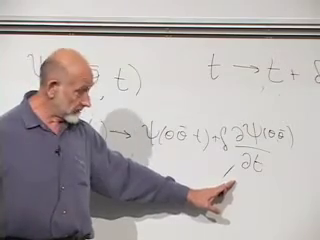
\includegraphics[width=0.72\textwidth]{lecture_05_figure_04.png}
\lectureframe{01:13:15.060}
\caption{Trên bảng, \(t\to t+\delta\) được đặt phía trên biến thiên bậc nhất của \(\Psi\), với hạng đạo hàm được chỉ ra trực tiếp.}
\end{figure}

\subsection{Tịnh tiến theo một hướng lẻ}

Bây giờ hãy nghĩ ra một phép biến đổi dịch một tọa độ lẻ:
\begin{equation}
\theta\longmapsto\theta+\epsilon,
\end{equation}
trong đó \(\epsilon\) là một tham số Grassmann lẻ khác. Đồng thời, cho thời gian nhận một độ dời lũy linh chẵn,
\begin{equation}
t\longmapsto t+i\bar\theta\epsilon.
\end{equation}
Cả \(\bar\theta\) lẫn \(\epsilon\) đều lẻ, nên tích của chúng là chẵn và có thể được cộng một cách nhất quán vào tọa độ chẵn \(t\).

Khi đưa tham số sang bên trái,
\begin{equation}
i\bar\theta\epsilon=-i\epsilon\bar\theta.
\end{equation}
Vì vậy biến thiên cảm sinh là
\begin{align}
\delta_\epsilon\Psi
&=\epsilon\,\partial_\theta\Psi
-i\epsilon\bar\theta\,\partial_t\Psi\\
&=\epsilon q_0\Psi,
\end{align}
trong đó
\begin{equation}
q_0=\partial_\theta-i\bar\theta\partial_t.
\end{equation}
Toán tử vi phân lẻ này là bộ sinh của phép dịch kết hợp. Một bộ sinh liên hợp tương thích, dùng các đạo hàm trái, là
\begin{equation}
\bar q_0=-\partial_{\bar\theta}
+i\theta\partial_t.
\end{equation}

Các dấu chính xác phụ thuộc vào việc dùng đạo hàm Grassmann trái hay phải, và vào cách phép liên hợp đảo ngược các thừa số lẻ. Điều không được phụ thuộc vào quy ước là sự khép kín trên phép tịnh tiến theo thời gian. Với các định nghĩa ở trên,
\begin{align}
\{q_0,\bar q_0\}
&=i\{\partial_\theta,\theta\}\partial_t
+i\{\bar\theta,\partial_{\bar\theta}\}\partial_t\\
&=2i\partial_t.
\end{align}
Hạng đạo hàm-đạo hàm triệt tiêu, cũng như hạng bậc hai theo các tọa độ lẻ. Hai hạng hỗn hợp mỗi hạng đều đóng góp \(i\partial_t\).

Vì \(H=i\partial_t\) trên các trạng thái trong ảnh Schrödinger,
\begin{equation}
\{q_0,\bar q_0\}=2H.
\end{equation}
Nếu ta chuẩn hóa
\begin{equation}
q=\frac{q_0}{\sqrt2},
\qquad
\bar q=\frac{\bar q_0}{\sqrt2},
\end{equation}
thì
\begin{equation}
\boxed{\{q,\bar q\}=H.}
\end{equation}
\editorialnote{Bài giảng cố ý đi qua các dấu chưa chắc chắn rồi sau đó nhận ra một hệ số 2. Quy ước đạo hàm trái được hiển thị bảo toàn phép tính trên lớp đó đồng thời cố định một chuẩn hóa tự nhất quán. Những quy ước chuẩn khác chuyển các dấu giữa các độ dời tọa độ và các bộ sinh.}

\begin{classroomqa}
\audiencequestion{Hệ số 2 cuối cùng trong phản giao hoán tử của siêu không gian xuất phát từ đâu? \lecturetimestamp{01:24:21}}
\lecturerresponse{Có hai đóng góp hỗn hợp bằng nhau. Một đến từ \(\{\partial_\theta,\theta\}=1\), và cái kia đến từ \(\{\partial_{\bar\theta},\bar\theta\}=1\). Mỗi cái nhân với đạo hàm theo thời gian. Vì vậy các bộ sinh chưa chuẩn hóa cho \(2i\partial_t\); một hệ số \(1/\sqrt2\) trong mỗi siêu điện tích khôi phục lại chuẩn hóa trước đó.}
\end{classroomqa}

\begin{classroomqa}
\audiencequestion{Việc xây dựng này có dùng giả thiết rằng \(\epsilon\) là nhỏ không? \lecturetimestamp{01:24:51}}
\lecturerresponse{Nó dùng tính lũy linh chứ không dùng một độ lớn số học thông thường. Vì \(\epsilon^2=0\), mọi khai triển theo một \(\epsilon\) đơn đều dừng sau bậc nhất. Gọi nó là vô cùng bé hay nhỏ là một phép loại suy hữu ích, nhưng sự cắt cụt là chính xác tuyệt đối.}
\end{classroomqa}

\editorialnote{Các tham số Grassmann không có độ lớn dương thông thường. Vai trò của chúng như các tham số vô cùng bé đến từ tính lũy linh và việc khai triển kết thúc chính xác.}

\subsection{Ý nghĩa hình học}

Đại số giờ đây có hai hiện thực tương đương. Trong bức tranh dao động tử, \(Q\) và \(\bar Q\) thay fermion bằng boson và boson bằng fermion. Trong bức tranh hình học, \(q\) và \(\bar q\) tịnh tiến một hàm theo các hướng lẻ đồng thời cảm sinh một độ dời thời gian thông thường. Trong cả hai bức tranh,
\begin{equation}
\begin{gathered}
\{\text{supercharge},\text{conjugate supercharge}\}\\
=\text{time-translation generator}.
\end{gathered}
\end{equation}

Không gian tọa độ tổng quát chứa \(t,\theta,\bar\theta\) là siêu không gian. Trong một lý thuyết trường tương đối tính, nó còn chứa các tọa độ không gian thông thường, và các siêu điện tích khép kín trên xung lượng không-thời gian đầy đủ \(P_\mu\), chứ không chỉ trên \(H=P_0\). Uốn cong cấu trúc này dẫn tới siêu hấp dẫn.

Trong một nghĩa, các biến Grassmann là một công cụ ghi sổ hiệu quả cho boson và fermion. Ở một nghĩa khác, hệ thức khép kín nói lên một điều sâu sắc hơn nhiều: sự phân biệt giữa loại hạt và hình học không-thời gian không còn là tuyệt đối. Di chuyển hai lần theo các hướng lẻ sinh ra chuyển động theo một hướng thông thường. Việc tự nhiên có hiện thực hóa cấu trúc đó bằng thực nghiệm hay không là chuyện tách biệt với sự kiện toán học rằng cấu trúc ấy là nhất quán, tiết kiệm và cứng một cách đáng kinh ngạc.
